\documentclass[border=4pt]{standalone}
\usepackage{amsmath,amssymb}
\usepackage{tikz}
\usetikzlibrary{arrows.meta,shadows,decorations.pathreplacing}
\begin{document}
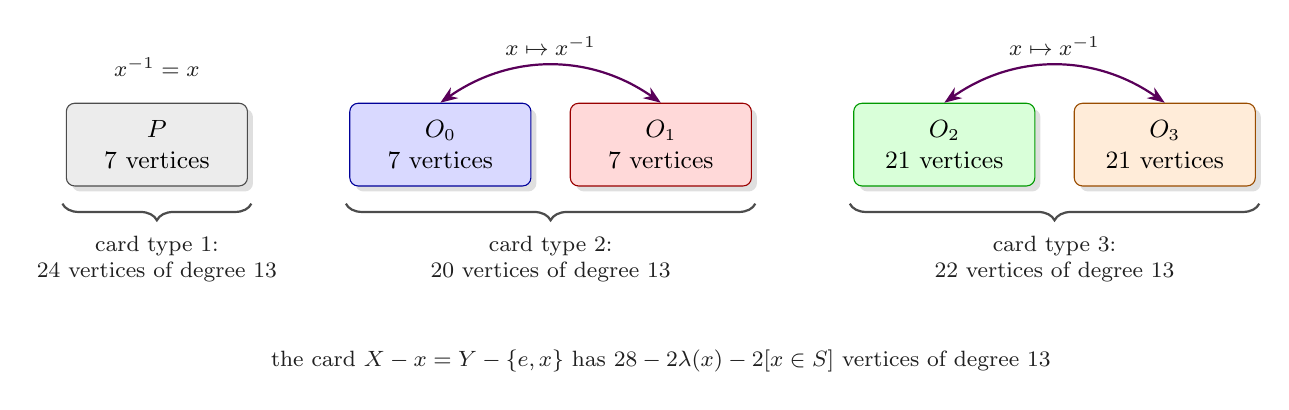
\begin{tikzpicture}[
  orb/.style={draw=#1!60!black,fill=#1!15,rounded corners=3pt,minimum width=2.3cm,minimum height=1.05cm,
              align=center,font=\small,
              drop shadow={opacity=0.25,shadow xshift=2pt,shadow yshift=-2pt}},
  >={Stealth[length=2.2mm]},
  inv/.style={<->,thick,violet!70!black},
  note/.style={font=\footnotesize,gray!25!black,align=center},
  br/.style={decorate,decoration={brace,amplitude=6pt,mirror},thick,gray!60!black}]
  \node[orb=gray]   (P)  at (0,0)    {$P$\\ $7$ vertices};
  \node[orb=blue]   (O0) at (3.6,0)  {$O_0$\\ $7$ vertices};
  \node[orb=red]    (O1) at (6.4,0)  {$O_1$\\ $7$ vertices};
  \node[orb=green]  (O2) at (10.0,0) {$O_2$\\ $21$ vertices};
  \node[orb=orange] (O3) at (12.8,0) {$O_3$\\ $21$ vertices};
  \draw[inv] (O0.north) to[bend left=35] node[above,note]{$x\mapsto x^{-1}$} (O1.north);
  \draw[inv] (O2.north) to[bend left=35] node[above,note]{$x\mapsto x^{-1}$} (O3.north);
  \node[note,above=6pt] at (P.north) {$x^{-1}=x$};
  \draw[br] (-1.2,-0.75) -- node[below=8pt,note]{card type 1:\\ $24$ vertices of degree $13$} (1.2,-0.75);
  \draw[br] (2.4,-0.75) -- node[below=8pt,note]{card type 2:\\ $20$ vertices of degree $13$} (7.6,-0.75);
  \draw[br] (8.8,-0.75) -- node[below=8pt,note]{card type 3:\\ $22$ vertices of degree $13$} (14.0,-0.75);
  \node[note] at (6.4,-2.75) {the card $X-x=Y-\{e,x\}$ has $28-2\lambda(x)-2[x\in S]$ vertices of degree $13$};
\end{tikzpicture}
\end{document}
